\section{Ebenen von Datenmodellen}
Das Modellieren effizienter Datenmodelle spielt in verschiedenen Arten von ICTs eine Rolle. Im folgenden Kapitel wird auf die für Planungs- und Designsysteme relevanten Modellierungen eingegangen. Es wird nicht auf andere Bereiche eingegangen in der Datenmodellierung eine Rolle spielt. Zum Beispiel wäre die Modellierung von Datenstrukturen und Protokollen die erlauben die Daten energiesparend zu verarbeiten, wie es unter anderem in einem Paper von Gang\cite{jour:Lu2007} vorgestellt wurde.

Für Planungs- und Designsysteme dienen dazu, die Betriebswirte in der Bewältigung von Problemen und der langfristigen Planung zu unterstützen. Diese Aufgabe werden in \cite{jour:Schulze2007} in kurzfristige sowie langfristige Planung aufgeteilt. Da sich die Aufgaben und die möglichen Aktionen unterscheiden, wird vorgeschlagen diese auf verschiedene Arten zu modellieren. Dabei werden die kurfristigen Aktionen in der operationalen Ebene, der \textit{Operational View}, und die langfristigen Aktionen in der analytischen Ebene, der \textit{Analytical View}, behandelt.

\begin{figure}[h]
 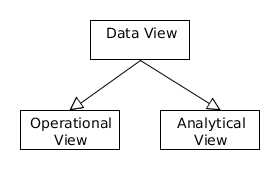
\includegraphics[natwidth=\textwidth]{figures/datamodelling/dataviews.png}
 \centering
 \caption{Sicht auf Daten. Operational View als Informationsquelle für taktische und Analytical View als Informationsquelle für strategische Entscheidungen.\cite{jour:Schulze2007}}
\end{figure}

\subsection{Operationale Ebene}





